\documentclass[12pt,a4paper]{report}
\usepackage[utf8]{inputenc}
\usepackage[spanish]{babel}
\usepackage{amsmath}
\usepackage{amsfonts}
\usepackage{amssymb}
\usepackage{makeidx}
\usepackage{graphicx}
\usepackage{lmodern}
\usepackage{kpfonts}
\usepackage[left=2cm,right=2cm,top=2cm,bottom=2cm]{geometry}
\author{Eduardo Robles}
\title{Par de Rotacion y Cuaternios}
\begin{document}
\begin{center}

\includegraphics[scale=1]{../../../../../../../Pictures/logo.png} 
\end{center}
\begin{flushright}

Ingeniería mecatrónica 7-A\\
Cinemática de Robots \\
Eduardo Robles Vázquez\\
Fecha: 17/Septiembre/2019\\
\end{flushright}
\paragraph{PAR DE ROTACIÓN Y CUATERNIOS}
\subparagraph{Par de rotación}
\begin{center}
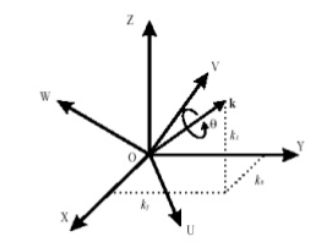
\includegraphics[scale=1]{../../../../../../../Pictures/2.png} 
\end{center}
\begin{flushleft}
La aplicación que se le da a un par de rotación es que rote un vector p a un ángulo theta alrededor del vector unitario k, esto se realiza a través de la siguiente expresión:\\
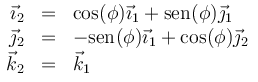
\includegraphics[scale=1]{../../../../../../../Pictures/1.png} 
\end{flushleft}
\subparagraph{Cuaternios}
\begin{flushleft}
Los cuaternios son una extensión de los números reales, parecidos a los números complejos. Mientras que los números complejos son una extensión de los reales por la adición de la unidad imaginaria i, los cuaternios son una extensión generada de manera análoga añadiendo las unidades imaginarias: i, j y k a los números reales.\\
La utilización de los cuaterniones para representar una rotación ofrece una gran ventaja puesto que se puede evitar el problema de singularidad, esto quiere decir que exista alguna indeterminación al querer rotar con un cierto ángulo.
\end{flushleft}
\begin{flushleft}
Bibliografía 
\end{flushleft}
@article{del1999representacion,
  title={La representaci{\'o}n de rotaciones mediante cuaterniones},
  author={del Castillo, GF Torres},
  journal={Miscelanea Matemtica},
  pages={43--50},
  year={1999}
}

\end{document}

